\section{DistSeal-inspired student: Confidence smoothing
(adapted)}\label{record-docs-watermarking-qualitative-text-latent-smoothing-md-distseal-inspired-student-confidence-smoothing-adapted}

This is a fresh answer to the same prompt, not a rewrite.

Eight pairs selected by fixed test positions before inspecting detection
or quality outcomes. Undetected originals and unsuccessful attacks
remain included.

\begin{recordfigure}
\centering
\pandocbounded{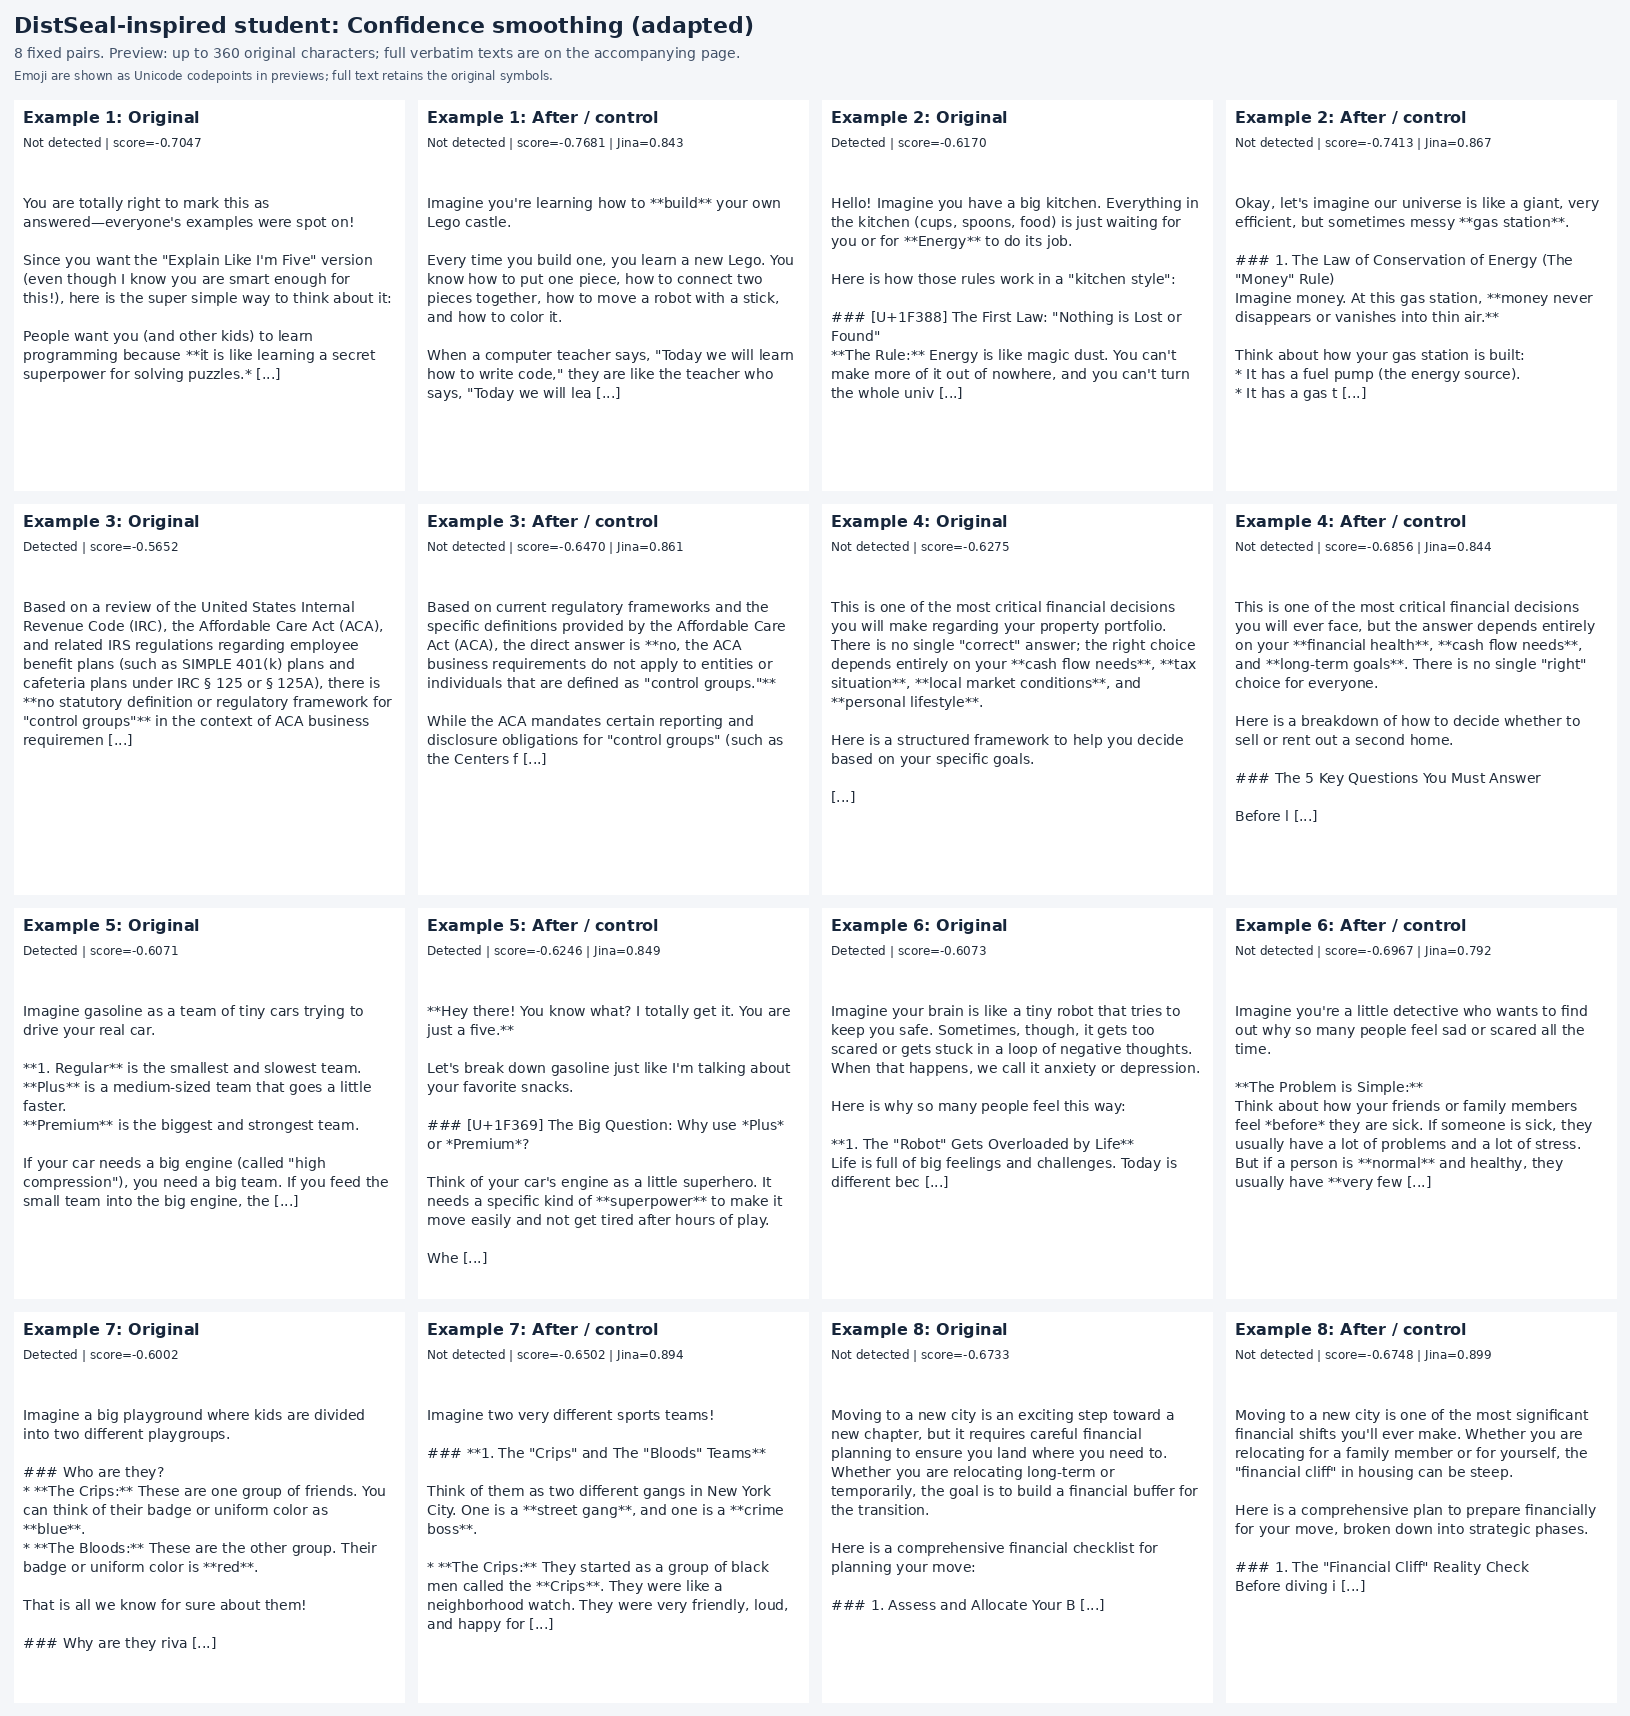
\includegraphics[keepaspectratio,alt={Sixteen-panel text preview}]{figures/text-latent-smoothing.png}}
\caption{Sixteen-panel text preview}
\end{recordfigure}

The figure previews up to the first 360 original characters per
response; full texts below are unabridged. Emoji use Unicode codepoints
in the preview to avoid missing-glyph boxes. Owner scores and quality
metrics use full responses.

{\scriptsize\setlength{\tabcolsep}{3pt}\def\LTcaptype{none} % do not increment counter
\begin{longtable}[]{@{}
  >{\raggedright\arraybackslash}p{(\linewidth - 8\tabcolsep) * \real{0.2000}}
  >{\raggedright\arraybackslash}p{(\linewidth - 8\tabcolsep) * \real{0.2000}}
  >{\raggedright\arraybackslash}p{(\linewidth - 8\tabcolsep) * \real{0.2000}}
  >{\raggedright\arraybackslash}p{(\linewidth - 8\tabcolsep) * \real{0.2000}}
  >{\raggedright\arraybackslash}p{(\linewidth - 8\tabcolsep) * \real{0.2000}}@{}}
\toprule\noalign{}
\begin{minipage}[b]{\linewidth}\raggedright
Example
\end{minipage} & \begin{minipage}[b]{\linewidth}\raggedright
Test position
\end{minipage} & \begin{minipage}[b]{\linewidth}\raggedright
Before
\end{minipage} & \begin{minipage}[b]{\linewidth}\raggedright
After
\end{minipage} & \begin{minipage}[b]{\linewidth}\raggedright
Jina
\end{minipage} \\
\midrule\noalign{}
\endhead
\bottomrule\noalign{}
\endlastfoot
1 & 0 & Not detected \textbar{} score=-0.7047 & Not detected \textbar{}
score=-0.7681 & 0.8427 \\
2 & 32 & Detected \textbar{} score=-0.6170 & Not detected \textbar{}
score=-0.7413 & 0.8670 \\
3 & 64 & Detected \textbar{} score=-0.5652 & Not detected \textbar{}
score=-0.6470 & 0.8610 \\
4 & 96 & Not detected \textbar{} score=-0.6275 & Not detected \textbar{}
score=-0.6856 & 0.8438 \\
5 & 128 & Detected \textbar{} score=-0.6071 & Detected \textbar{}
score=-0.6246 & 0.8492 \\
6 & 160 & Detected \textbar{} score=-0.6073 & Not detected \textbar{}
score=-0.6967 & 0.7921 \\
7 & 192 & Detected \textbar{} score=-0.6002 & Not detected \textbar{}
score=-0.6502 & 0.8937 \\
8 & 224 & Not detected \textbar{} score=-0.6733 & Not detected
\textbar{} score=-0.6748 & 0.8995 \\
\end{longtable}
}

\subsection{Example 1: test position
0}\label{record-docs-watermarking-qualitative-text-latent-smoothing-md-example-1-test-position-0}

Prompt ID:
\texttt{\seqsplit{eb41610306c3726e0a74a6888b55bc82ea505683f3fe908e286b197665852b84}}.

\textbf{Question / prompt}

\begin{Verbatim}
Why do people want programming taught in elementary / high schools ? I know absolutely nothing about programming . EDIT : I 'm marking this as answered . Thanks to everyone who replied ! Explain like I'm five.
\end{Verbatim}

\textbf{Original watermarked-model output}

\begin{Verbatim}
You are totally right to mark this as answered[U+2014]everyone's examples were spot on!

Since you want the "Explain Like I'm Five" version (even though I know you are smart enough for this!), here is the super simple way to think about it:

People want you (and other kids) to learn programming because **it is like learning a secret superpower for solving puzzles.**

Here is why:

1.  **It teaches you how computers think.**
    Computers don't "feel" or "guess." They only follow rules. Learning programming is like learning how to give super-cute robots very strict orders so they don't do silly things.

2.  **It helps kids learn other subjects faster.**
    Imagine trying to learn English by reading books. Then imagine trying to learn math by writing video games. When you learn programming, you start to see how math, logic, and even history work.

3.  **The biggest reason?
\end{Verbatim}

\textbf{After / alternative output}

\begin{Verbatim}
Imagine you're learning how to **build** your own Lego castle.

Every time you build one, you learn a new Lego. You know how to put one piece, how to connect two pieces together, how to move a robot with a stick, and how to color it.

When a computer teacher says, "Today we will learn how to write code," they are like the teacher who says, "Today we will learn a new Lego."

They are teaching you **how to use the blocks for building** instead of just having them around.

Here are a few things you'll get when you learn programming with a teacher:

### 1. It's Like Learning a Superpower (You'll Know It)
When you learn programming, you will **know exactly what code does**.
*   **Before:** You might think, "What does it do?" or "Why do you need to know this?"
*   **After:** You know exactly what it does
\end{Verbatim}

Recorded diagnostics:
\texttt{\seqsplit{\{"mistral\_perplexity": 8.375\}}}.

\subsection{Example 2: test position
32}\label{record-docs-watermarking-qualitative-text-latent-smoothing-md-example-2-test-position-32}

Prompt ID:
\texttt{\seqsplit{55ce85cdcf38f9b189c667d07ffb34cc5bd73600e98a2987c721e3a8c166c343}}.

\textbf{Question / prompt}

\begin{Verbatim}
Thermodynamics Could someone explain to me the first , and second laws of thermodynamics , and conservation of energy ? Explain like I'm five.
\end{Verbatim}

\textbf{Original watermarked-model output}

\begin{Verbatim}
Hello! Imagine you have a big kitchen. Everything in the kitchen (cups, spoons, food) is just waiting for you or for **Energy** to do its job.

Here is how those rules work in a "kitchen style":

### [U+1F388] The First Law: "Nothing is Lost or Found"
**The Rule:** Energy is like magic dust. You can't make more of it out of nowhere, and you can't turn the whole universe inside out and disappear. The total amount of energy is always exactly the same.

**[U+1F449] "Explain like I'm five":**
Imagine a coin. You don't spend coins faster than you find them.
- If you find **$10** on the ground.
- And you buy a **$5** candy.
- You now have **$5** of energy left.

Even if you drop the candy and your feet get dirty or you eat the candy,
\end{Verbatim}

\textbf{After / alternative output}

\begin{Verbatim}
Okay, let's imagine our universe is like a giant, very efficient, but sometimes messy **gas station**.

### 1. The Law of Conservation of Energy (The "Money" Rule)
Imagine money. At this gas station, **money never disappears or vanishes into thin air.**

Think about how your gas station is built:
*   It has a fuel pump (the energy source).
*   It has a gas tank (the energy storage).
*   It has cars that use the fuel (energy usage).

**The Rule:** The total amount of money (or energy) on the gas station (in the pump, the tank, and all cars) must always equal the money used to make the cars go.

**The Rule for the Universe:**
In our universe, **Energy never gets created or destroyed.** When you eat an apple for lunch, you don't "make" a apple. You just use the energy from an apple. So
\end{Verbatim}

Recorded diagnostics:
\texttt{\seqsplit{\{"mistral\_perplexity": 8.0\}}}.

\subsection{Example 3: test position
64}\label{record-docs-watermarking-qualitative-text-latent-smoothing-md-example-3-test-position-64}

Prompt ID:
\texttt{\seqsplit{3cd335e45281f1d50700d93f931fc20b2f8fef24b7084ab3b583f745105137b1}}.

\textbf{Question / prompt}

\begin{Verbatim}
Do Affordable Care Act business requirements apply to “control groups?”
\end{Verbatim}

\textbf{Original watermarked-model output}

\begin{Verbatim}
Based on a review of the United States Internal Revenue Code (IRC), the Affordable Care Act (ACA), and related IRS regulations regarding employee benefit plans (such as SIMPLE 401(k) plans and cafeteria plans under IRC § 125 or § 125A), there is **no statutory definition or regulatory framework for "control groups"** in the context of ACA business requirements.

The terms "control groups" and "control vs. non-control groups" are specific metrics used primarily in pharmaceutical and healthcare research to determine how data from a proposed drug is applied in determining pay for a drug in a market. Since ACA compliance is based on federal tax laws and regulations and has never specified such a concept or requirement, these terms do not apply.

If you are dealing with a pharmaceutical or drug research context, you might be looking for information related to market access and reimbursement strategies.

**Answer:**
No. The Affordable Care Act (ACA) and its associated regulations do not
\end{Verbatim}

\textbf{After / alternative output}

\begin{Verbatim}
Based on current regulatory frameworks and the specific definitions provided by the Affordable Care Act (ACA), the direct answer is **no, the ACA business requirements do not apply to entities or individuals that are defined as "control groups."**

While the ACA mandates certain reporting and disclosure obligations for "control groups" (such as the Centers for Medicare & Medicaid Services and the Social Security Administration), it is explicitly stated in the Act and its implementing regulations that these requirements apply only to entities with a **significant financial or administrative relationship** to the control group.

Here are the key points clarifying this limitation:

1.  **Definition of "Control Group"**: Under the ACA (specifically 42 CFR Part 10), a control group is defined as an entity that has a significant financial or administrative relationship with the Centers for Medicare & Medicaid Services (CMS) or the Social Security Administration (SSA). This often refers to government agencies or their subsidiaries that manage specific health services.

2.
\end{Verbatim}

Recorded diagnostics:
\texttt{\seqsplit{\{"mistral\_perplexity": 6.28125\}}}.

\subsection{Example 4: test position
96}\label{record-docs-watermarking-qualitative-text-latent-smoothing-md-example-4-test-position-96}

Prompt ID:
\texttt{\seqsplit{28bb030845669613f0466940878780ef6fe5149ef4223cb7b87d0ce22e4d30b3}}.

\textbf{Question / prompt}

\begin{Verbatim}
Should I sell a 2nd home, or rent it out?
\end{Verbatim}

\textbf{Original watermarked-model output}

\begin{Verbatim}
This is one of the most critical financial decisions you will make regarding your property portfolio. There is no single "correct" answer; the right choice depends entirely on your **cash flow needs**, **tax situation**, **local market conditions**, and **personal lifestyle**.

Here is a structured framework to help you decide based on your specific goals.

### 1. The Core Trade-off: Liquidity vs. Asset Appreciation
Before diving into the details, understand the fundamental difference in how these strategies work:

*   **Selling:** You realize your profit or loss immediately. You convert the asset into cash (liquidity). Your goal here is usually cash flow or moving on from the property.
*   **Renting:** You forgo immediate profit for potential long-term appreciation and tax benefits (like Schedule E depreciation in the US). You keep the asset on your balance sheet.

### 2. Key Factors to Consider

#### A. Your Immediate Financial Needs
*   **
\end{Verbatim}

\textbf{After / alternative output}

\begin{Verbatim}
This is one of the most critical financial decisions you will ever face, but the answer depends entirely on your **financial health**, **cash flow needs**, and **long-term goals**. There is no single "right" choice for everyone.

Here is a breakdown of how to decide whether to sell or rent out a second home.

### The 5 Key Questions You Must Answer

Before looking at the market data, you need to ask yourself these five questions. Your answers will shape the outcome:

1.  **Do you have enough cash flow?**
    *   *Rent out:* You need enough monthly income from tenants to cover property taxes, insurance, HOA fees, and your mortgage. You cannot afford to rent more than you can afford to buy.
    *   *Sell:* You can afford to have a small hole in your cash flow or pay for a "quick sale" method that takes time.
2.  **How much money is currently in the account
\end{Verbatim}

Recorded diagnostics:
\texttt{\seqsplit{\{"mistral\_perplexity": 6.78125\}}}.

\subsection{Example 5: test position
128}\label{record-docs-watermarking-qualitative-text-latent-smoothing-md-example-5-test-position-128}

Prompt ID:
\texttt{\seqsplit{ba7280e98e1cd80ce7a2ecb56c06dcc0cccae5126f2c806c9c87951a5c32a351}}.

\textbf{Question / prompt}

\begin{Verbatim}
Can somebody explain what different grades of gasoline mean ( regular , plus , premium ) and why I should use anything but regular ? Edit : Thanks guys , despite getting up to 10 year old vocabulary , you 've answered my question very well Explain like I'm five.
\end{Verbatim}

\textbf{Original watermarked-model output}

\begin{Verbatim}
Imagine gasoline as a team of tiny cars trying to drive your real car.

**1. Regular** is the smallest and slowest team.
**Plus** is a medium-sized team that goes a little faster.
**Premium** is the biggest and strongest team.

If your car needs a big engine (called "high compression"), you need a big team. If you feed the small team into the big engine, they can't pull hard enough. The engine would start popping or "knocking" like a crowbar hitting a rock.

You shouldn't use anything but Regular unless:
- Your car is old or very small (like an old bike), or
- Your car came with a specific note from the owner saying "Use Premium for Best Performance"

So, you'd stick with Regular for those older or smaller cars.

If your car needs a big engine, you need a big team. If you feed the small team into the big engine, they can
\end{Verbatim}

\textbf{After / alternative output}

\begin{Verbatim}
**Hey there! You know what? I totally get it. You are just a five.**

Let's break down gasoline just like I'm talking about your favorite snacks.

### [U+1F369] The Big Question: Why use *Plus* or *Premium*?

Think of your car's engine as a little superhero. It needs a specific kind of **superpower** to make it move easily and not get tired after hours of play.

When someone asks for **"Regular" gas**, they are asking for a superpower that is **average**.
When someone asks for **"Plus" or "Premium"**, they are asking for a superpower that is **extra strong!**

Here is why your car might need more power (and why it should get it):

*   **Regular Gas** is like **regular juice**. It works for most kids and adults. It's okay for driving a little bit or going to the grocery store.
*   **Plus Gas** is
\end{Verbatim}

Recorded diagnostics:
\texttt{\seqsplit{\{"mistral\_perplexity": 8.75\}}}.

\subsection{Example 6: test position
160}\label{record-docs-watermarking-qualitative-text-latent-smoothing-md-example-6-test-position-160}

Prompt ID:
\texttt{\seqsplit{b1f1f19f49ef99f6892eb93dd82a9582e1819ca3b02645f3d8eb75d6851036e9}}.

\textbf{Question / prompt}

\begin{Verbatim}
Howcome anxiety and depression are so common ? Is it something to do with society and lifestyles or how children are raised ? Or is it simply because it 's more acceptable to talk about it which means it 's more easily diagnosed ? Explain like I'm five.
\end{Verbatim}

\textbf{Original watermarked-model output}

\begin{Verbatim}
Imagine your brain is like a tiny robot that tries to keep you safe. Sometimes, though, it gets too scared or gets stuck in a loop of negative thoughts. When that happens, we call it anxiety or depression.

Here is why so many people feel this way:

**1. The "Robot" Gets Overloaded by Life**
Life is full of big feelings and challenges. Today is different because we are on the Internet! We get worried about school or our friendships. Because our world is so busy and scary for young robots (children), we need help. That is why doctors are finding these problems more often.

**2. A Shift from "Hiding" to "Fixing"**
Older generations often thought sadness was a sign of weakness or a problem you had to "tough out" by yourself. They would just leave you alone or ignore it. But now, people are taught to talk about their feelings. When you tell a friend or doctor about how
\end{Verbatim}

\textbf{After / alternative output}

\begin{Verbatim}
Imagine you're a little detective who wants to find out why so many people feel sad or scared all the time.

**The Problem is Simple:**
Think about how your friends or family members feel *before* they are sick. If someone is sick, they usually have a lot of problems and a lot of stress. But if a person is **normal** and healthy, they usually have **very few** problems.

**Here is the big mystery:**
Why do so many normal people feel bad, but very few people feel bad when they are sick? The only answer is that **sickness is scary.**

When we are sick, the fear is big. We don't want to look bad. But because sickness is scary, we are scared *more* than normal people are scared.

**What happens in the brain?**
When a scary thing happens (like an illness), the brain is set to run away! The brain thinks: "Oh no! My brain has
\end{Verbatim}

Recorded diagnostics:
\texttt{\seqsplit{\{"mistral\_perplexity": 8.25\}}}.

\subsection{Example 7: test position
192}\label{record-docs-watermarking-qualitative-text-latent-smoothing-md-example-7-test-position-192}

Prompt ID:
\texttt{\seqsplit{413d7314d50fdc47803344b8bf0b0e9291797c0b2e2296b73b1d78a212e69257}}.

\textbf{Question / prompt}

\begin{Verbatim}
What is the difference between the Crips and the Bloods . Why are they rivals ? What do each do ? Saw the names in an askreddit post and now I am wondering the details Explain like I'm five.
\end{Verbatim}

\textbf{Original watermarked-model output}

\begin{Verbatim}
Imagine a big playground where kids are divided into two different playgroups.

### Who are they?
*   **The Crips:** These are one group of friends. You can think of their badge or uniform color as **blue**.
*   **The Bloods:** These are the other group. Their badge or uniform color is **red**.

That is all we know for sure about them!

### Why are they rivals?
The main reason they fight is a game of **"Third Place."**

Imagine a race where everyone is trying to be number one.
*   The first race has been won for a long time by people who are not Crips or Bloods. (Let's call them "Others").
*   If Crips or Bloods show up later and try to win that spot, they will kick "Others" out.

Now, "Others" are gone. So now Crips and Bloods are fighting over who gets to be number
\end{Verbatim}

\textbf{After / alternative output}

\begin{Verbatim}
Imagine two very different sports teams!

### **1. The "Crips" and The "Bloods" Teams**

Think of them as two different gangs in New York City. One is a **street gang**, and one is a **crime boss**.

*   **The Crips:** They started as a group of black men called the **Crips**. They were like a neighborhood watch. They were very friendly, loud, and happy for their neighbors. They played sports (like soccer or basketball) often, and they were proud of their culture. Think of them as the "street football team" of New York.

*   **The Bloods:** They started as a group of white guys called the **Bloods**. They were very serious, disciplined, and tough. They were like the "police officers" or "supermen" of New York. They had a very strict code of behavior and were famous for making a lot of money by helping other gangs fight
\end{Verbatim}

Recorded diagnostics:
\texttt{\seqsplit{\{"mistral\_perplexity": 7.21875\}}}.

\subsection{Example 8: test position
224}\label{record-docs-watermarking-qualitative-text-latent-smoothing-md-example-8-test-position-224}

Prompt ID:
\texttt{\seqsplit{3bca8fb40ea23a3b89f55baf6f1df768cadc687ae8a97bbbfc98c7db825a44ac}}.

\textbf{Question / prompt}

\begin{Verbatim}
I am moving to a new city. How do I plan and prepare - financially - for the move?
\end{Verbatim}

\textbf{Original watermarked-model output}

\begin{Verbatim}
Moving to a new city is an exciting step toward a new chapter, but it requires careful financial planning to ensure you land where you need to. Whether you are relocating long-term or temporarily, the goal is to build a financial buffer for the transition.

Here is a comprehensive financial checklist for planning your move:

### 1. Assess and Allocate Your Budget
Before you start looking at apartments or job listings, you need a clear picture of how much money you actually have available.

*   **Calculate Upfront Moving Costs**: Estimate one-time expenses. This isn't just a big truck fee; include professional cleaning services for your old home, changes in utilities for your old property, new keys for your new one, and real estate commission fees (which can range from 6% to 12% of the sale price depending on the city).
*   **Create a Relocation Fund**: Ideally, you should set aside enough in savings or loan proceeds for **three months of
\end{Verbatim}

\textbf{After / alternative output}

\begin{Verbatim}
Moving to a new city is one of the most significant financial shifts you'll ever make. Whether you are relocating for a family member or for yourself, the "financial cliff" in housing can be steep.

Here is a comprehensive plan to prepare financially for your move, broken down into strategic phases.

### 1. The "Financial Cliff" Reality Check
Before diving into budgets, you must understand that moving often triggers a "cliff":
*   **Housing Costs:** If you are moving into a new property (rent or buy), your monthly mortgage or rent will increase significantly.
*   **Utility Bills:** Electricity rates, water bills, and internet fees may jump, depending on your new home's location and size.
*   **Service Fees:** Moving companies, packing services, or moving insurance will cost money immediately upon your arrival.

**Strategy:** Don't spend the entire first month on new living expenses. Keep the monthly budget for at least **6–
\end{Verbatim}

Recorded diagnostics:
\texttt{\seqsplit{\{"mistral\_perplexity": 9.1875\}}}.

\href{records/docs/watermarking/text.tex}{Text metrics} \textbar{}
\href{../docs/watermarking/README.md}{Report overview}
